\documentclass[a4paper, 12pt]{article}
\usepackage{comment} % enables the use of multi-line comments (\ifx \fi) 
\usepackage{lipsum} %This package just generates Lorem Ipsum filler text. 
\usepackage{fullpage} % changes the margin
\usepackage[a4paper, total={7in, 10in}]{geometry}
\usepackage{amsmath}
\usepackage{amssymb,amsthm}  % assumes amsmath package installed
\newtheorem{theorem}{Theorem}
\newtheorem{corollary}{Corollary}
\usepackage{graphicx}
\usepackage{tikz}
\usepackage{quiver}
\usepackage{setspace}
%\usepackage{enumitem}
\usetikzlibrary{arrows}
\usepackage{verbatim}
\usepackage[shortlabels]{enumitem}

\usepackage{float}
\usepackage{tikz-cd}


    
\usepackage{xcolor}
\usepackage{mdframed}
\usepackage[shortlabels]{enumitem}
%\usepackage{indentfirst}
\usepackage{hyperref}
    
\renewcommand{\thesubsection}{\thesection.\alph{subsection}}


\newenvironment{problem}[2][Problem]
    { \begin{mdframed}[backgroundcolor=gray!20] \textbf{#1 #2} \\}
    {  \end{mdframed}}

\newenvironment{background}
{\begin{center}
    \begin{tabular}{|p{\textwidth}|}
    \hline\\
    }
    { 
    \\\\\hline
    \end{tabular} 
    \end{center}}
% Define solution environment
\newenvironment{solution}
    {\textit{Solution:}}
    {}

%Define the claim environment
\newenvironment{claim}[1]{\par\noindent\underline{Claim:}\space#1}{}
\newenvironment{claimproof}[1]{\par\noindent\underline{Proof:}\space#1}{\hfill $\blacksquare$}

\renewcommand{\qed}{\quad\qedsymbol}
\newcommand{\rank}{\text{rank}\,}
\newcommand{\im}{\text{Im}\,}
\newcommand{\la}{\langle}
\newcommand{\ra}{\rangle}
%%%%%%%%%%%%%%%%%%%%%%%%%%%%%%%%%%%%%%%%%%%%%%%%%%%%%%%%%%%%%%%%%%%%%%%%%%%%%%%%%%%%%%%%%%%%%%%%%%%%%%%%%%%%%%%%%%%%%%%%%%%%%%%%%%%%%%%%
\begin{document}
%Header-Make sure you update this information!!!!
\noindent
%%%%%%%%%%%%%%%%%%%%%%%%%%%%%%%%%%%%%%%%%%%%%%%%%%%%%%%%%%%%%%%%%%%%%%%%%%%%%%%%%%%%%%%%%%%%%%%%%%%%%%%%%%%%%%%%%%%%%%%%%%%%%%%%%%%%%%%%
\large\textbf{Zhengdong Zhang} \hfill \textbf{Homework 2}   \\
Email: zhengz@uoregon.edu \hfill ID: 952091294 \\
\normalsize Course: MATH 635 - Algebraic Topology II \hfill Term: Winter 2025\\
Instructor: Dr.Daniel Dugger \hfill Due Date: $25^{th}$ January, 2025 \\
\noindent\rule{7in}{2.8pt}
\setstretch{1.1}


\begin{problem}{2}
Calculate the homology groups of \(\mathbb{R}P^2\# T\) and identify which compact 2-manifold it is.
\end{problem}
\begin{solution}
Let \(X=\mathbb{R}P^2\# T\) and consider the following cellular structure on \(X\):
\[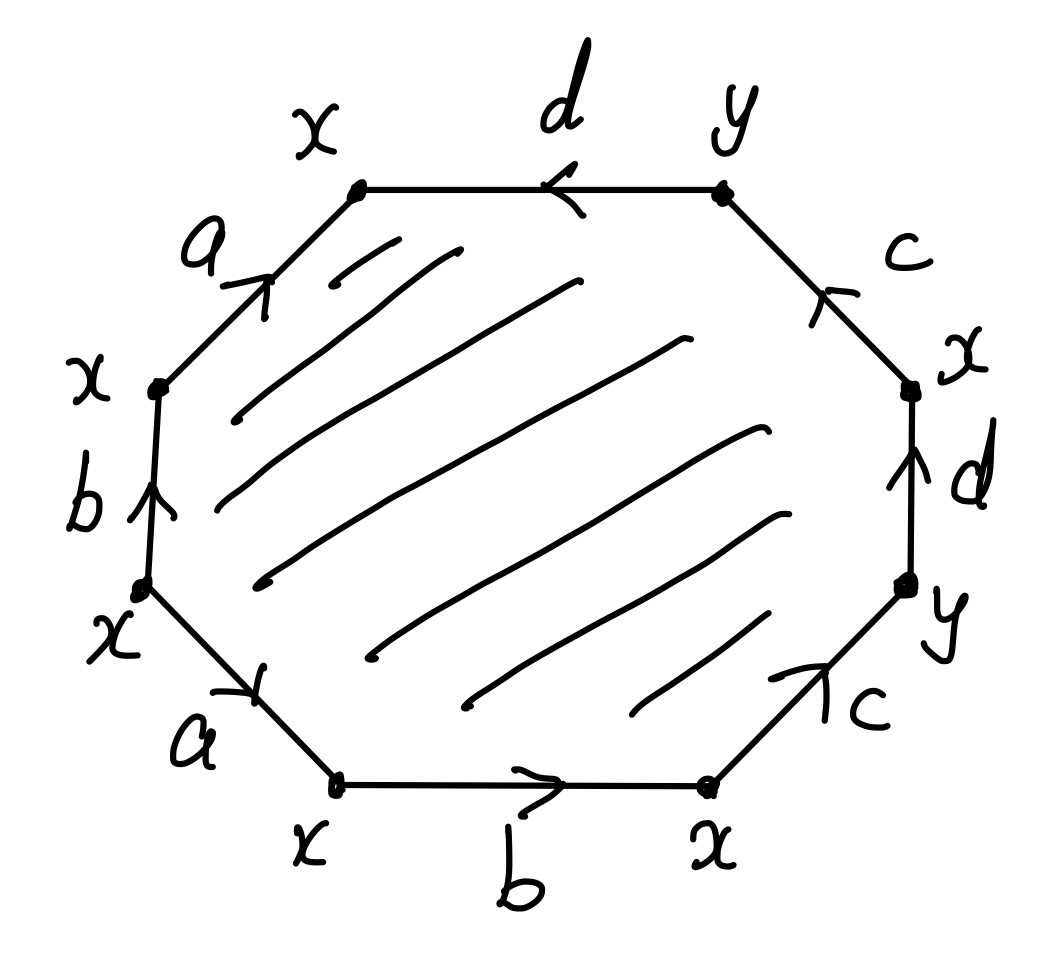
\includegraphics[scale=0.15]{Pictures/HW2p.jpg}\]
The space \(X\) has two 0-cells \(x,y\), four 1-cells \(a,b,c,d\) and one 2-cell \(S\). We have the following cellular chain complex:
\[\mathbb{Z}\xrightarrow{d_2}\mathbb{Z}^4\xrightarrow{d_1}\mathbb{Z}^2\xrightarrow{d_0} 0.\]
The boundary maps are given by 
\begin{align*}
    d_2(S)&=2c+2d,\\ 
    d_1(a)=d_1(b)&=0,\\ 
    d_1(c)=-d_1(d)&=y-x.
\end{align*} 
So the homology can be calculated as follows 
\[H_2(X)=\ker d_2=0.\]
and 
\begin{align*}
H_0(X)&=\ker d_0/\im d_1\\ 
      &=\la x,y\ra/\la y-x\ra\\ 
      &=\mathbb{Z}.
\end{align*}
\begin{align*}
H_1(X)&=\ker d_1/\im d_2\\ 
      &=\la a,b,c+d\ra/\la 2c+2d\ra\\ 
      &=\mathbb{Z}\oplus \mathbb{Z}\oplus \mathbb{Z}/2 \mathbb{Z}.
\end{align*}
The homology groups of \(X\) can be summarized as follows: 
\[H_i(X)=\begin{cases}
    \mathbb{Z},&\, \text{if}\, i=0;\\ 
    \mathbb{Z}^2\oplus \mathbb{Z}/2 \mathbb{Z},&\, \text{if}\, i=1;\\
    0,&\, \text{otherwise}. 
\end{cases}\]
By comparing the calculations in problem 1, we can see that \(X\) has the same homology groups as \(\mathbb{R}P^2\#\mathbb{R}P^2\#\mathbb{RP}^2\), so 
\(\mathbb{R}P^2\# T\) must be homeomorphic to \(\mathbb{R}P^2\#\mathbb{R}P^2\#\mathbb{R}P^2\). 
\end{solution}






\end{document}